\documentclass[sigconf,nonacm]{acmart}
\usepackage{booktabs}
\usepackage{array}
\usepackage{tikz}
\usetikzlibrary{arrows.meta,positioning,fit}
\usepackage{pgfplots}
\pgfplotsset{compat=1.18}
\usepackage{balance}

\definecolor{hnavy}{HTML}{112B45}
\definecolor{hblue}{HTML}{1E78B4}
\definecolor{hgreen}{HTML}{167C63}
\definecolor{hpale}{HTML}{EAF4F8}
\definecolor{hred}{HTML}{A4423D}
\setlength{\textfloatsep}{7pt plus 2pt minus 2pt}
\setlength{\floatsep}{6pt plus 2pt minus 2pt}
\setlength{\intextsep}{6pt plus 2pt minus 2pt}
\renewcommand{\arraystretch}{1.06}
\setlength{\emergencystretch}{1em}
\settopmatter{printacmref=false}
\setcopyright{none}
\renewcommand\footnotetextcopyrightpermission[1]{}

\title{Horizon: Evidence-Conditioned Runtime Assurance for Autonomous Maritime Systems}
\author{Tan Wee Joe}
\affiliation{%
  \institution{University College London}
  \city{London}
  \country{United Kingdom}}
\email{tanweejoe@gmail.com}

\begin{document}
\begin{abstract}
Horizon inserts an independent safety governor between a vessel's decision-making AI and its actuators. It joins navigation, contact, platform, communication, perception, and neural-health evidence before passing, modifying, replacing, or rejecting each proposed command. A 60-episode development study compared five candidates across four encounter classes. No declared-recoverable branch collided and no unsafe or stale decision passed the independent gate. We select A5, an evidence-conditioned predictive and barrier-filter hybrid, for the hackathon prototype: it achieved 99.83\% gate acceptance with three deadline misses. This is an engineering choice, not a certified ranking; all missions were censored, 40 branches exceeded an assumed uncertainty bound, and only three paired seeds were run per scenario.
\end{abstract}
\ccsdesc[500]{Computer systems organization~Robotic autonomy}
\ccsdesc[300]{Computing methodologies~Computer vision}
\keywords{runtime assurance, autonomous maritime systems, safety governor, mechanistic interpretability, sparse autoencoder}
\maketitle

\section{Safety Objective}
Autonomous maritime systems can emit unsafe commands even when individual components appear healthy. Horizon therefore enforces one protected actuation path. The external AI proposes a command but cannot write to steering or propulsion. Assurance evaluates public observations and declared uncertainty; an exclusive gate revalidates identity, lineage, epoch, freshness, deadline, actuator limits, and final-command safety. A watchdog retains minimum-risk authority if supervision stops.

The governing rule is monotone: unknown, stale, invalid, unbounded, or late evidence may only preserve or reduce authority. Camera or neural evidence is a \emph{perception-health input}, not proof of obstacle-free water.

\begin{figure}[t]
\centering
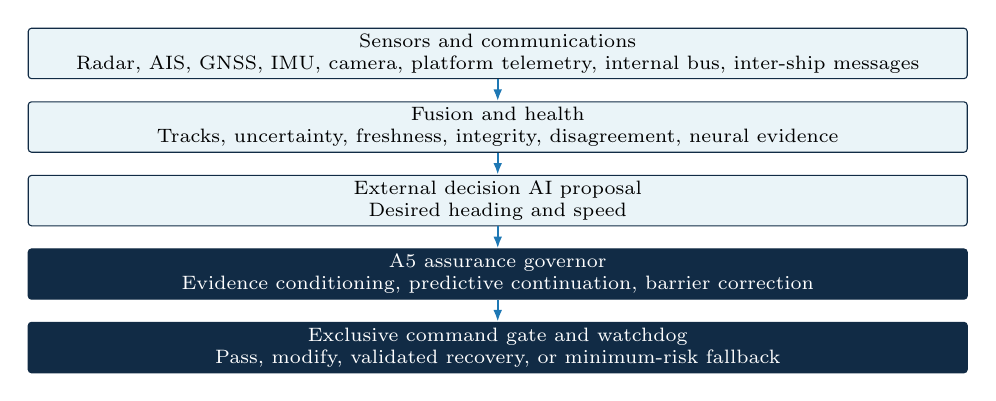
\begin{tikzpicture}[node distance=2.8mm, every node/.style={font=\scriptsize,align=center}, box/.style={draw=hnavy,rounded corners=1.2pt,minimum width=\columnwidth-2mm,minimum height=5.7mm,inner sep=2pt}, arr/.style={-{Latex[length=1.5mm]},hblue,thick}]
\node[box,fill=hpale] (sense) {Sensors and communications\\Radar, AIS, GNSS, IMU, camera, platform telemetry, internal bus, inter-ship messages};
\node[box,fill=hpale,below=of sense] (fusion) {Fusion and health\\Tracks, uncertainty, freshness, integrity, disagreement, neural evidence};
\node[box,fill=hpale,below=of fusion] (ai) {External decision AI proposal\\Desired heading and speed};
\node[box,fill=hnavy,text=white,below=of ai] (a5) {A5 assurance governor\\Evidence conditioning, predictive continuation, barrier correction};
\node[box,fill=hnavy,text=white,below=of a5] (gate) {Exclusive command gate and watchdog\\Pass, modify, validated recovery, or minimum-risk fallback};
\draw[arr] (sense)--(fusion); \draw[arr] (fusion)--(ai); \draw[arr] (ai)--(a5); \draw[arr] (a5)--(gate);
\end{tikzpicture}
\caption{Protected Horizon control path. Evaluation truth is isolated from this path.}
\label{fig:architecture}
\end{figure}

\section{Candidate Architectures}
All candidates implement one bounded input-to-decision contract. A1 applies CPA/TCPA thresholds and Simplex switching. A2 uses an uncalibrated analytic Gaussian collision-risk approximation with Simplex recovery. A3 requires finite rollout and a complete recovery continuation. A4 searches a nonlinear vessel plant map for a barrier-compatible command and validates it with a full 3DOF rollout. A5 conditions bounds and speed on evidence health, attempts predictive recoverability, and invokes A4 when required.

\subsection{A5 decision path}
Healthy evidence retains nominal bounds and a 6\,m/s cap; degraded evidence expands bounds by 1.5 and caps speed at 3\,m/s; invalid evidence caps speed at 1\,m/s and forces recovery. A5 checks the request through a short handoff and complete recovery continuation. If that fails, it applies A4 and validates the correction with a complete rollout. Incomplete, infeasible, late, or unsupported results fall back to recovery or minimum-risk control.

\section{Experimental Method}
The matrix contained 12 paired identities: four scenarios, three seeds, and five candidates per identity, for 60 branches. Scenarios covered recoverable crossing, dense traffic, vessel degradation, and initially-unrecoverable encounters. Each branch ran for 30 simulated seconds under the idealized timing profile. Exact joins linked evaluation, diagnostics, and assumption audits; all collisions, timeouts, bound violations, and censored outcomes remained in their denominators~\cite{a32}.

\begin{table}[b]
\centering
\caption{A1--A5 development results.}
\label{tab:results}
\scriptsize
\begin{tabular}{@{}lrrrr@{}}
\toprule
 & Gate & Deadline & Recoverable & Unsafe/stale\\
ID & accepted & misses & collisions & accepted\\
\midrule
A1 & 8.87\% & 0  & 0 & 0\\
A2 & 8.73\% & 1  & 0 & 0\\
A3 & 99.66\% & 6 & 0 & 0\\
A4 & 99.44\% & 10 & 0 & 0\\
\textbf{A5} & \textbf{99.83\%} & \textbf{3} & \textbf{0} & \textbf{0}\\
\bottomrule
\end{tabular}
\end{table}

\section{Results and Architecture Choice}
All 15 branches in the deliberately unrecoverable stratum collided; none of the 45 declared-recoverable branches collided. No unsafe or stale result was accepted by the gate. A1 and A2 were computationally light but mostly passed proposals that the independent gate later rejected, giving acceptance rates below 9\%. A3--A5 actively selected recovery or minimum-risk actions and exceeded 99.4\% acceptance. A5 recorded the highest acceptance and fewer deadline misses than A3 or A4 (Fig.~\ref{fig:controller}). We therefore recommend A5 for the hackathon integration while retaining A1 as the transparent baseline.

\begin{center}
\centering
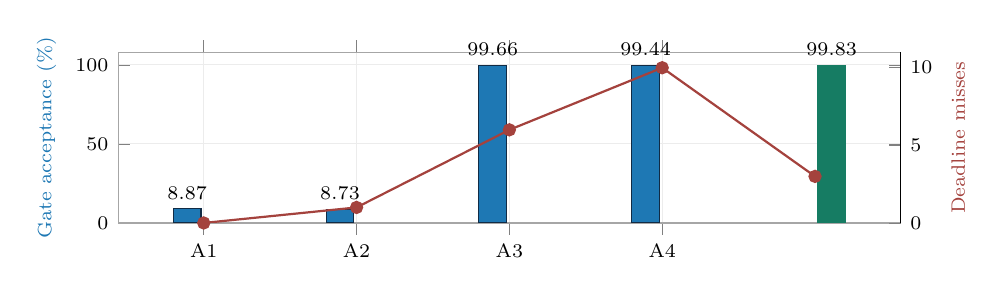
\begin{tikzpicture}
\begin{axis}[
  name=accept,width=.95\columnwidth,height=3.75cm,
  ybar,bar width=10pt,ymin=0,ymax=108,
  symbolic x coords={A1,A2,A3,A4,A5},xtick=data,
  ylabel={Gate acceptance (\%)},ylabel style={hblue},
  nodes near coords,nodes near coords style={font=\scriptsize},
  tick label style={font=\scriptsize},label style={font=\scriptsize},
  axis line style={draw=gray!70},grid=major,grid style={gray!15},
  enlarge x limits=.14]
\addplot[fill=hblue,draw=hnavy] coordinates {(A1,8.87) (A2,8.73) (A3,99.66) (A4,99.44)};
\addplot[fill=hgreen,draw=hgreen] coordinates {(A5,99.83)};
\end{axis}
\begin{axis}[
  at={(accept.south west)},anchor=south west,
  width=.95\columnwidth,height=3.75cm,
  axis x line=none,axis y line*=right,
  ymin=0,ymax=11,
  symbolic x coords={A1,A2,A3,A4,A5},xtick=data,
  ylabel={Deadline misses},ylabel style={hred},
  tick label style={font=\scriptsize},label style={font=\scriptsize},
  enlarge x limits=.14]
\addplot[hred,thick,mark=*,mark options={fill=hred}] coordinates {(A1,0) (A2,1) (A3,6) (A4,10) (A5,3)};
\end{axis}
\end{tikzpicture}
\captionof{figure}{Gate acceptance (bars) and candidate deadline misses (red markers), 12 branches per candidate. Counts are descriptive, not a formal safety ranking.}
\label{fig:controller}
\end{center}

\section{Neural Mechanistic Evidence}
The implemented mechanistic-interpretability experiment is H4: a small sparse autoencoder (SAE) fitted to all 2,048 spatially pooled encoder channels from WaSR-T's ResNet-101 \texttt{layer4}. Inputs are standardized and encoded into 16 nonnegative ReLU features. Runtime novelty would be the standardized reconstruction mean-square error plus an $L_1$ sparsity term. The 296-frame development fit reached its 3,000-epoch cap, reducing loss from 0.992552 to 0.168764 with zero dead features, but it did not meet the convergence criterion~\cite{perception}.

For exploratory causal testing, the largest adjacent-frame SAE-code change was selected independently for three predeclared frame pairs. Its decoder direction was injected into the real \texttt{layer4} activation during six-frame temporal replay. The measured output was the absolute change in mean obstacle-class logit inside MODD2 obstacle boxes. Each selected direction exceeded both a random-direction and equal-norm noise control (Fig.~\ref{fig:causal}), but the absolute effects were small and the selection was pair-specific.

\begin{center}
\centering
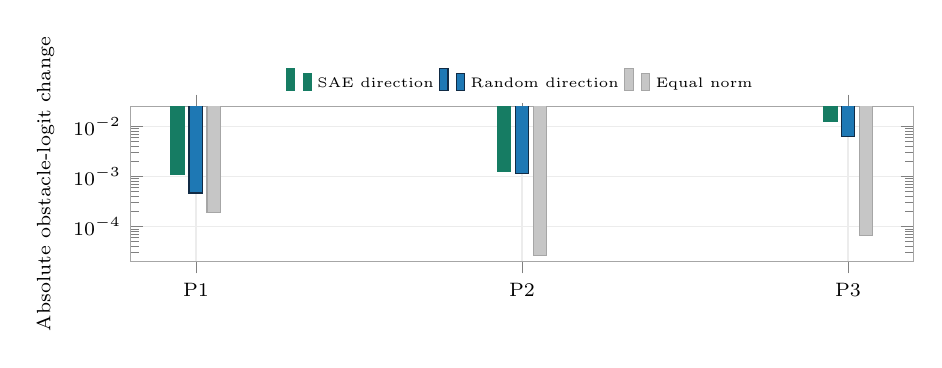
\begin{tikzpicture}
\begin{axis}[
 width=.95\columnwidth,height=3.55cm,
 ybar=1.5pt,bar width=5pt,ymode=log,ymin=0.00002,ymax=0.025,
 symbolic x coords={P1,P2,P3},xtick=data,
 ylabel={Absolute obstacle-logit change},
 legend style={font=\tiny,at={(0.5,1.02)},anchor=south,legend columns=3,draw=none},
 tick label style={font=\scriptsize},label style={font=\scriptsize},
 grid=major,grid style={gray!15},axis line style={draw=gray!70}]
\addplot[fill=hgreen,draw=hgreen] coordinates {(P1,0.001119) (P2,0.001281) (P3,0.012779)};
\addplot[fill=hblue,draw=hnavy] coordinates {(P1,0.000466) (P2,0.001163) (P3,0.006381)};
\addplot[fill=gray!45,draw=gray!70] coordinates {(P1,0.000191) (P2,0.0000267) (P3,0.0000670)};
\legend{SAE direction,Random direction,Equal norm}
\end{axis}
\end{tikzpicture}
\captionof{figure}{Offline H4 causal probes on three development pairs. Log scale.}
\label{fig:causal}
\end{center}

H4 is \emph{not deployed as a trusted runtime sensor}. Its claim gate remains closed because the SAE did not converge, the experiment used one sequence and one seed, no stable maritime semantic was assigned, and calibration and held-out partitions remain unopened. The live recorded-camera service currently defaults to H0 output entropy and permits H0/H1 only. H4 code therefore returns \texttt{unknown} unless a frozen causal-validation artifact explicitly passes the claim gate. This fail-closed boundary prevents exploratory interpretation from silently increasing camera authority.

\section{Limitations and Next Study}
The experiment cannot support certification or a final ranking. All 60 missions were censored, so route completion and cost are unknown. Forty branches exceeded an engineering uncertainty bound. No independent recovery boundary was supplied, front-end delay was idealized, and gate/watchdog actions affected trajectories. Three seeds per scenario are insufficient for statistical claims.

The next study should freeze methods before opening held-out data; run at least 1,000 paired episodes with 30 or more seeds per stochastic cell; separate preventable and unrecoverable encounters; validate perception thresholds on target CUDA hardware; and measure sensor-to-actuator latency. Deployment also requires qualified hydrodynamics, uncertainty coverage, communication-fault tests, and real ship interfaces.

\section{Conclusion}
Horizon demonstrates a coherent pattern: diverse ship and AI evidence informs a bounded governor while an independent gate owns actuation and fails closed. A5 is the best current hackathon architecture because it combines evidence-conditioned margins, predictive continuation, plant-aware correction, and the strongest measured acceptance/miss balance. SAE reconstruction and activation intervention remain exploratory until convergence, calibration, and held-out causal replication close the claim gate.

\balance
\begin{thebibliography}{9}
\scriptsize
\bibitem{a32} Horizon Project, ``A32 A1--A5 30-second development analysis,'' revision \texttt{28eb923}, Sept. 2026, analysis hash \texttt{8004358e...e909}.
\bibitem{perception} Horizon Project, ``MODD2 development evidence and extraction completion,'' Sept. 2026.
\bibitem{wasrt} L. Zust et al., ``WaSR-T official implementation,'' \url{https://github.com/lojzezust/WaSR-T}.
\bibitem{modd2} B. Bovcon et al., ``MODD2 maritime obstacle-detection dataset,'' \url{https://github.com/bborja/modd}.
\end{thebibliography}

\end{document}
